\documentclass[report.tex]{subfiles}

\begin{document}

\section{Úloha E}\label{sec:E}

\subsection{Spracovanie všeobecnej triedy pre $L^1$ a $L^{\infty}$ regresiu}

Vypracovali sme modul \pyth|Model| pre počítanie $L^1$ a $L^{\infty}$ regresie z ľubovoľných číselných dát, ktorý využíva LP formulácie popísané vyššie. Konkrétne \pyth|L1Model| využíva formuláciu na minimalizovanie $L^1$ normy a \pyth|LInfModel| minimalizuje $L^{\infty}$ normu. Príklad použitia tohto modelu sa nachádza v \verb|model_demonstration.ipynb| Následne opíšeme jednotlivé metódy jednotlivých modelov.

\subsubsection*{\pyth|Model.__init__(dependent_vect, independent_vect)|}

Konštruktor triedy, spoločný pre oba modely, vytvorí inštanciu, ktorá si drží dáta a vie na nich vykonávať operácie popísané nižšie. 

Argumenty:

\begin{itemize}
	\item \pyth|dependent_vect: np.ndarray| - vektor závislých premenných
	\item \pyth|independent_vect: np.ndarray| - matica, ktorej riadky sú vektory nezávislých premenných
\end{itemize}

\subsubsection*{\pyth|Model.solve()|}

Metóda, ktorá vyrieši regresnú LP úlohu na daných dátach. \pyth|L1Model.solve()| rieši minimalizáciou $L^1$ normy a \pyth|LInfModel.solve()|, rieši minimalizáciou $L^{\infty}$ normy. 

Vracia:

\begin{itemize}
	\item \pyth|np.ndarray| - vektor optimálnych $\beta$ premenných
\end{itemize}

Po zavolaní tejto metódy si inštancia uloží vektor optimálnych $\beta$ premenných do atribútu \pyth|self._beta|, potrebné pre metódy popísané nižšie.

\subsubsection*{\pyth|Model.r2()|}

Vypočíta $R^2$ koeficient pre dané dáta a vypočítaný vektor $\beta$.

Vracia:

\begin{itemize}
	\item \pyth|float| - výsledný $R^2$ koeficient
\end{itemize}

\subsubsection*{\pyth|Model.visualize()|}

Ak je počet nezávislých premenných 1 alebo 2, táto metóda vykreslí graf dát spolu s vypočítanou regresnou priamkou, resp. rovinou. 

Vracia:

\begin{itemize}
	\item \pyth|bool| - úspešnosť vizualizácie, kde \pyth|False| označuje, že nezávislých premenných je viac ako 2, čiže nie je možné vykresliť graf
\end{itemize}

\subsection{Porovnanie použitia $L^1$ a $L^{\infty}$ lineárnej regresie}

\textit{Nasledujúce tvrdenia popisujú len naše pozorovania správania sa jednotlivých lineárnych regresii na generovaných dátach}

Vyššie v sekcii \ref{sec:A} sme ukázali, že implementácie lineárnej regresie pomocou merania vzdialenost $L^1$ a $L^{\infty}$ normou majú optimálne riešenie, pre ľubovoľné vstupné dáta. Snažili sme sa odpozorovať, ako sa jednotlivé prístupy odlišujú pre nejaké konkrétne dáta.

V dátach, v ktorých je výrazná lineárna závislosť, minimalizovanie $L^1$ normy veľmi dobre zachytáva práve tento lineárny vzťah, aj v prítomnosti odľahlých dát - outlierov. Toto správanie vie ale viesť aj k tzv. \textit{overfittingu}. Model príliš tesne zachytáva takéto správanie, čo môže viesť k horším odhadom pre budúce pozorovania.

Na druhej strane minimalizovanie $L^{\infty}$ normy je veľmi ovplyvňované outliermi. Aj pre \enquote{jasne} lineárne dáta s nejakými chybnými pozorovaniami, tieto dátové body výrazne odklonia regresnú priamku/nadrovinu. 

\subsubsection{Minimalizácia váženého súčtu}

Toto správanie $L^{\infty}$ lineárnej regresie môžeme využiť na zníženie overfittingu $L^1$ lineárnej regresie. Jeden z možných prístupov môže byť napríklad pomocou minimalizácie váženej sumy $\omega||y - \hat{y}||_1 + (1-\omega)||y - \hat{y}||_{\infty},~\omega \in [0;1]$. Formulovaná LP úloha vyzerá nasledovne (značenie sme prebrali z \eqref{P1} a \eqref{Pinf}):	


\begin{align*}
	\text{min}~ &
	\left(
	\begin{array}{c|c|c}
		\mathbf{0}_{k+1}^T & \omega\mathbf{1}_n^T & (1 - \omega)
	\end{array}
	\right)
	\left(
	\begin{array}{c}
		\beta \\
		\hline
		t \\
		\hline
		\gamma
	\end{array}
	\right) \\
	&\left(
	\begin{array}{c|c|c}
		\mathbf{A} & \mathbb{I}_n & \mathbf{0}_n \\
		\hline
		-\mathbf{A} & \mathbb{I}_n & \mathbf{0}_n \\
		\hline
		\mathbf{A} & \mathbf{0}_{n \times n} & \mathbf{1}_n \\
		\hline
		-\mathbf{A} & \mathbf{0}_{n \times n} & \mathbf{1}_n \\
	\end{array}
	\right)
	\left(
	\begin{array}{c}
		\beta \\
		\hline
		t \\
		\hline
		\gamma
	\end{array}
	\right)
	\geq
	\left(
	\begin{array}{c}
		y \\
		\hline
		-y \\
		\hline
		y \\
		\hline
		-y
	\end{array}
	\right) \\
	&\beta \in \mathbb{R}^{k+1},~t \geq \mathbf{0}_{n},~\gamma \geq 0
\end{align*}

Podobným spôsobom ukážeme, že táto úloha nadobúda optimálne riešenie. Sformulujme duálnu úlohu:

\begin{align*}
	\text{Nech}~&\alpha = \left(
	\begin{array}{c}
		\alpha_1 \\
		\hline
		\alpha_2 \\
		\hline
		\alpha_3 \\
		\hline
		\alpha_4
	\end{array}
	\right),~\alpha_{1,2,3,4} \in \mathbb{R}^n
	\\
	\text{max}~ &
	\left(
	\begin{array}{c|c|c|c}
		y^T & -y^T & y^T & -y^T
	\end{array}
	\right)
	\alpha \\
	&\left(
	\begin{array}{c|c|c|c}
		\mathbf{A}^T & -\mathbf{A}^T & \mathbf{A}^T & -\mathbf{A}^T
	\end{array}
	\right)
	\alpha
	=
	\mathbf{0}_{k+1} \\
	&\left(
	\begin{array}{c|c|c|c}
		\mathbb{I}_n & \mathbb{I}_n & \mathbf{0}_{n \times n} & \mathbf{0}_{n \times n}
	\end{array}
	\right)
	\alpha
	\leq
	\omega \mathbf{1}_{n} \\
	&\left(
	\begin{array}{c|c|c|c}
		\mathbf{0}_n^T & \mathbf{0}_n^T & \mathbf{1}_{n}^T & \mathbf{1}_{n}^T
	\end{array}
	\right)
	\alpha
	\leq
	1-\omega\\
	&\alpha \geq \mathbf{0}_{4n} 
\end{align*}

Vidíme, že primárna úloha je prípustná pre $\beta = \mathbf{0}_{k+1},~t=|y|,~\gamma=|\hat{y}|$ (využitím značenia ako v \ref{sec:1Optim} a \ref{sec:InfOptim}) a duálna úloha je prípustná pre $\alpha = \mathbf{0}_{4n}$, teda zo silnej duality obe riešenia nadobúdajú optimálne riešenie.

\newpage

\subsubsection{Implementácia \pyth|WeightedL1LInfModel|}

Takáto lineárna regresia je implementovaná v triede \pyth|WeightedL1LInfModel|. Jej používanie je rovnaké ako pri predchádzajúcich implementáciách. Jediná zmena je pre metódu \pyth|WeightedL1LInfModel.solve(omega)|, ktorá teraz očakáva parameter \pyth|omega: float| v intervale $[0;1]$.


\begin{figure}[h!]
	\centering
	\begin{subfigure}[b]{0.48\linewidth}
		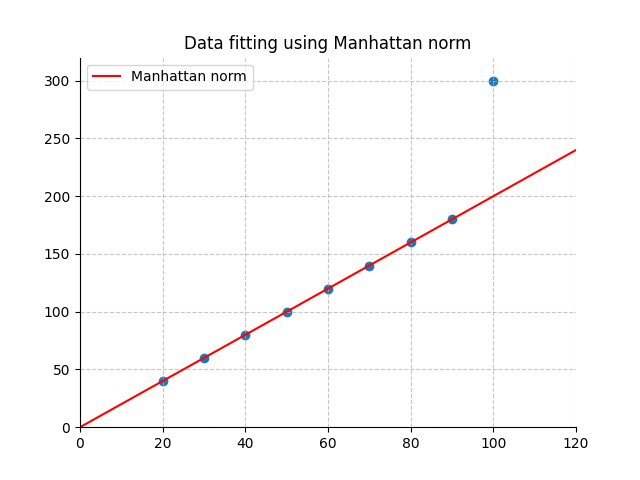
\includegraphics[width=\linewidth]{figs/L1_linear_with_outlier.png}
	\end{subfigure}
	\begin{subfigure}[b]{0.48\linewidth}
	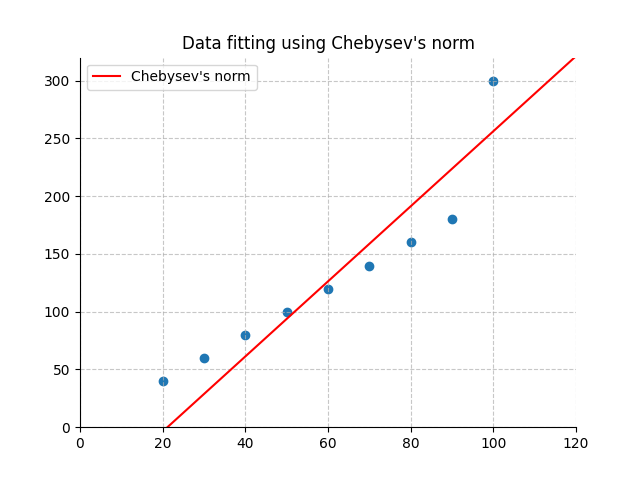
\includegraphics[width=\linewidth]{figs/LInf_linear_with_outlier.png}
	\end{subfigure}
	\begin{subfigure}[b]{0.48\linewidth}
		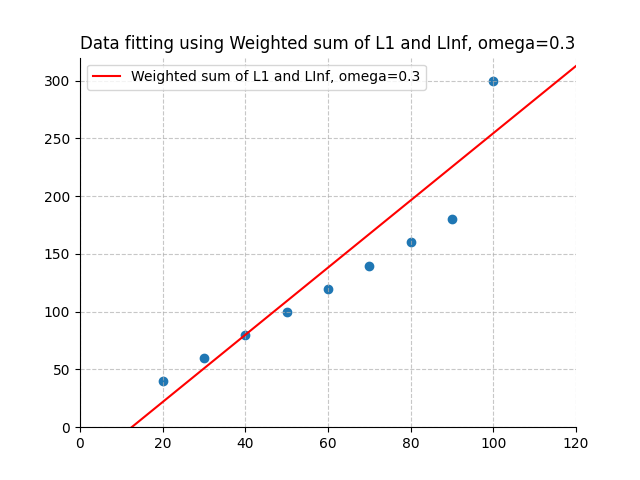
\includegraphics[width=\linewidth]{figs/weighted_linear_with_outlier.png}
	\end{subfigure}
	\begin{subfigure}[b]{0.48\linewidth}
		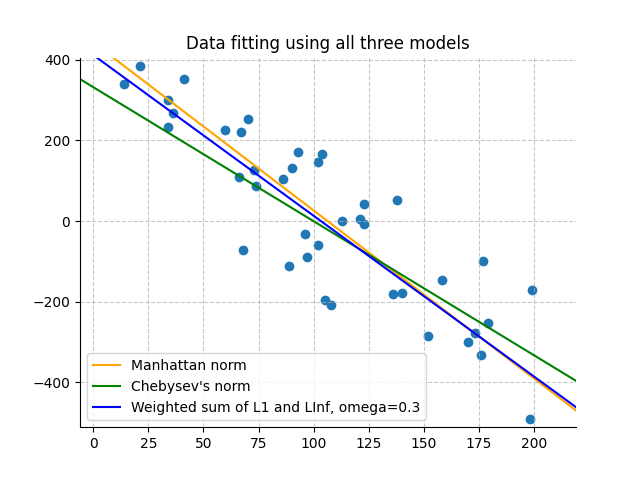
\includegraphics[width=\linewidth]{figs/all_three_random.png}
	\end{subfigure}
	\caption*{\centering Porovnanie správania sa jednotlivých regresii, prvé tri grafy zobrazujú rovnaké lineárne dáta s jedným outlierom}
\end{figure}

\end{document}